% =============================================================================
%  Internship Report -- single-file standalone version
%  Author: Raman Kapoor, ABV-IIITM Gwalior
%  Logo: ABV_IIITM_Logo.jpeg next to this .tex (graceful fallback if absent)
% =============================================================================
\documentclass[12pt,a4paper,oneside]{report}

% ---------- Encoding & fonts ----------
\usepackage[utf8]{inputenc}
\usepackage[T1]{fontenc}
\usepackage{lmodern}
\usepackage{mathptmx}

% ---------- Layout ----------
\usepackage[margin=1in,top=1in,bottom=1in,left=1.25in,right=1in]{geometry}
\usepackage{fancyhdr}
\usepackage{titlesec}
\usepackage{setspace}
\onehalfspacing

% ---------- Content ----------
\usepackage{graphicx}
\usepackage{enumitem}
\usepackage{booktabs}
\usepackage{longtable}
\usepackage{makecell}
\usepackage{multirow}
\usepackage{multicol}
\usepackage{caption}
\usepackage{subcaption}
\usepackage{url}

% ---------- Code & math ----------
\usepackage{amsmath}
\usepackage{amssymb}
\usepackage{listings}
\usepackage{tikz}
\usetikzlibrary{shapes.geometric, arrows.meta, positioning, calc, patterns}
\usepackage{xcolor}
\usepackage{float}

% ---------- Hyperref last ----------
\usepackage[hidelinks]{hyperref}
\hypersetup{
    colorlinks=true,
    linkcolor=black,
    citecolor=blue!60!black,
    urlcolor=blue!60!black,
    pdftitle={Internship Report -- Raman Kapoor},
    pdfauthor={Raman Kapoor}
}

% ---------- Headers ----------
\renewcommand{\chaptermark}[1]{\markboth{\chaptername\ \thechapter.\ #1}{}}
\renewcommand{\sectionmark}[1]{\markright{\thesection.\ #1}}
\pagestyle{fancy}
\fancyhf{}
\fancyhead[L]{\nouppercase{\scriptsize\bfseries\leftmark}}
\fancyhead[R]{\nouppercase{\scriptsize\bfseries\rightmark}}
\fancyfoot[C]{\bfseries\thepage}
\renewcommand{\headrulewidth}{0.4pt}
\setlength{\headheight}{15pt}

% ---------- Chapter heading ----------
\titleformat{\chapter}[display]
  {\normalfont\Large\bfseries}
  {\chaptertitlename\ \thechapter}{12pt}{\Large}
  [\vspace{0.2cm}\noindent\rule{\textwidth}{0.4pt}]
\titlespacing*{\chapter}{0pt}{-20pt}{20pt}

% ---------- Listings ----------
\definecolor{codegreen}{rgb}{0,0.5,0}
\definecolor{codegray}{rgb}{0.5,0.5,0.5}
\definecolor{codepurple}{rgb}{0.58,0,0.82}
\definecolor{backcolour}{rgb}{0.96,0.96,0.96}
\lstdefinestyle{nice}{
    backgroundcolor=\color{backcolour},
    commentstyle=\color{codegreen},
    keywordstyle=\color{blue}\bfseries,
    numberstyle=\tiny\color{codegray},
    stringstyle=\color{codepurple},
    basicstyle=\ttfamily\footnotesize,
    breakatwhitespace=false,
    breaklines=true,
    captionpos=b,
    keepspaces=true,
    numbers=left,
    numbersep=5pt,
    showspaces=false,
    showstringspaces=false,
    showtabs=false,
    tabsize=2,
    frame=single
}
\lstset{style=nice}

% =============================================================================
\begin{document}
\setcounter{page}{1}
\pagenumbering{roman}

% ============================== TITLE PAGE ===================================
\begin{titlepage}
\thispagestyle{empty}
\begin{center}
\fontsize{15.8pt}{19pt}\selectfont
{\textbf{Internship Report:\\Distributed Infrastructure and Backend Engineering\\at Juspay and Namma Yatri\\}}
\vspace*{0.15in}
\emph{\large{A report submitted for end-term evaluation of the internship for the award of}} \\
\emph{\large{Bachelor of Technology}} \\
\large{in} \\
\large{Information Technology}\\[0.3cm]
\large{By}\\
\large{\textbf{Raman Kapoor : 2022BIT-XXX}} \\[0.4cm]
\large{Under the Mentorship of} \\
\large{\textbf{Pranshu Anand}} \\
\large{(Industry Mentor, Juspay)}\\[0.3cm]
\large{Faculty Advisor:\,\textbf{Dr.\ Vivek Kumar Singh}}
\end{center}

\vspace{0.6cm}
\begin{center}
\IfFileExists{ABV_IIITM_Logo.jpeg}{%
    
\includegraphics[width=3cm]{ABV_IIITM_Logo.jpeg}%
}{%
    \fbox{\parbox[c][3cm][c]{3cm}{\centering\small[ABV-IIITM\\logo]}}%
}
\end{center}

\begin{center}
{\large{ABV-INDIAN INSTITUTE OF INFORMATION TECHNOLOGY}}\\[0.05cm]
{\large{AND MANAGEMENT GWALIOR}}\\[0.1cm]
{\large{GWALIOR, INDIA}}\\[0.1cm]
{\large{2026}}
\end{center}
\end{titlepage}

% ============================== DECLARATION ==================================
\thispagestyle{empty}
\begin{center}
{\Large \bf DECLARATION}
\end{center}
\vspace{0.5cm}
\noindent I hereby certify that the work, which is being presented in the report entitled INTERNSHIP REPORT: DISTRIBUTED INFRASTRUCTURE AND BACKEND ENGINEERING AT JUSPAY AND NAMMA YATRI, in fulfillment of the requirement for end-term evaluation of the internship for the award of the degree of Bachelor of Technology in Information Technology and submitted to the institution is an authentic record of my own work carried out under the mentorship of Mr.\ Pranshu Anand (Juspay) and the academic guidance of Dr.\ Vivek Kumar Singh. I also cited the references about the text(s)/figure(s)/table(s) from where they have been taken.

\vspace{1cm}
\begin{center}
\begin{tabular}{p{0.58\textwidth}p{0.4\textwidth}}
Dated:  & {\bf{Signature of the candidate}} \\
\end{tabular}
\end{center}

\vspace{1.5cm}
\noindent This is to certify that the above statement made by the candidate is correct to the best of my knowledge.

\vspace{1.5cm}
\begin{center}
\begin{tabular}{p{0.65\textwidth}p{0.4\textwidth}}
Dated: & {\bf{Signature of faculty advisor}} \\
\end{tabular}
\end{center}
\clearpage

% ============================ ACKNOWLEDGEMENT ================================
\thispagestyle{empty}
\begin{center}
{\LARGE \bf Acknowledgements}
\end{center}
\noindent
I would like to express my sincere gratitude to my industry mentor at \emph{Juspay}, Mr.\ Pranshu Anand, for the technical depth and the scope of ownership he extended to me during this internship. The work spanned distributed block storage, in-process caching for payment APIs, and a Shamir-secret-sharing-based secrets infrastructure --- each a substantial engineering challenge in its own right --- and his trust in letting me drive these projects end-to-end was the single biggest source of my growth this year.

I am equally grateful to the maintainers and contributors of \emph{Namma Yatri}, the open-source ride-hailing platform on which I designed and shipped the distributed event-driven payout scheduler. The depth of the public review process, the rigour of the production constraints, and the willingness of the community to engage seriously with intern-led contributions were genuinely unusual and shaped how I now think about correctness in distributed systems.

I would also like to acknowledge my faculty advisor at ABV-IIITM Gwalior, Dr.\ Vivek Kumar Singh, for his continual support and supervision over the course of this internship and the parallel B.Tech project, and for the freedom he gave me to pursue ideas that crossed the boundary between industry practice and academic enquiry.

Finally, I thank my family and friends for their unwavering encouragement, and the faculty and staff of ABV-IIITM Gwalior for the academic environment that made this work possible.

\begin{flushright}
\textit{\textbf{Raman Kapoor}}
\end{flushright}
\clearpage

% ============================== ABSTRACT =====================================
\thispagestyle{empty}
\begin{center}
{\Large\bf Abstract}
\end{center}
\noindent This report presents the work undertaken across two production engineering engagements and one self-directed cloud-infrastructure project during the internship year. The first engagement, as a \textbf{Software Developer Intern at Juspay}, comprised three projects on the production payments platform: (i) replacing CEPH-based block storage with \textbf{Lightbits NVMe/TCP}, achieving 4$\times$ storage efficiency by delivering 48{,}000 TPS over 4 nodes versus 37{,}000 TPS over 40 nodes while enabling active-active high-availability for Barbican via a shared backend; (ii) implementing a \textbf{thread-level and server-local caching} layer for high-traffic payment APIs that reduced cross-node network calls by over 4\,\% at peak and cut p95 latency by 11.2\,\%, while preserving correctness through formal cache-safety boundaries; and (iii) designing a \textbf{distributed secrets infrastructure} based on Shamir secret sharing, memory-only keys, and Raft-based replication, replacing heavy AWS KMS usage. The second engagement, as a \textbf{Backend Engineer (Open Source) at Namma Yatri}, delivered a distributed event-driven payout scheduling system that reduced driver payout latency from weekly cycles to T+2 hours under real production traffic of 10{,}000+ rides per day, backed by a Redis-based delayed job scheduler with per-ride locking and idempotent state management. The third workstream, a self-directed project on \textbf{PostgreSQL on Kubernetes/OpenStack}, architected a five-layer nested virtualisation stack on a single i9-14900 host, automated HA cluster provisioning end-to-end with Cluster API and CloudNativePG, and shipped a Zero-Trust secret-delivery framework using a Go-based OpenBao broker and a custom Python SDK. Together, these projects span block storage, in-process caching, distributed secrets, event-driven scheduling, and cloud automation --- providing comprehensive exposure to production-grade distributed-systems engineering.
\clearpage

% ============================== TOC + LoF + LoT ==============================
\tableofcontents
\clearpage
\listoffigures
\clearpage
\listoftables
\clearpage

% ============================== BODY (arabic) ================================
\setcounter{page}{1}
\pagenumbering{arabic}

% ----------------------------- CHAPTER 1: INTRODUCTION ----------------------
\chapter[Introduction]{Introduction and Overview}
\label{chap:intro}

\section{Internship Overview}

This internship spanned two distinct industry engagements and one self-directed cloud-infrastructure project, each contributing to a different stratum of the modern distributed-systems stack.

\begin{itemize}[leftmargin=*]
    \item \textbf{Juspay} (Software Developer Intern, January 2026 -- Present): production payments platform handling tens of thousands of transactions per second across the Indian fintech ecosystem. Three projects were delivered here, all on production traffic: a block-storage migration from CEPH to Lightbits NVMe/TCP, a two-tier in-process caching layer for high-traffic APIs, and a Shamir-secret-sharing-based replacement for AWS KMS.
    \item \textbf{Namma Yatri} (Backend Engineer, Open Source, November 2025 -- January 2026): the open-source ride-hailing platform serving Indian cities, written in Haskell with PostgreSQL and Redis. Contributed a distributed, event-driven payout scheduling system for special zones, serving 10{,}000+ rides daily.
    \item \textbf{Self-directed} (Personal Infrastructure, March 2026): a five-layer nested virtualisation stack on a single workstation that exercises OpenStack, Kubernetes, CloudNativePG, and OpenBao end-to-end, automating HA Postgres provisioning and Zero-Trust secret delivery.
\end{itemize}

\section{Themes}

Three recurring themes connect these otherwise unrelated projects:

\begin{enumerate}[leftmargin=*]
    \item \textbf{Correctness under concurrency.} Whether the system in question is a payment API, a ride payout scheduler, or a multi-tenant secret store, the correctness boundary is the same: never duplicate a chargeable event, never lose a write, never serve stale data when authoritative state is required. This report repeatedly returns to the techniques that enforce that boundary --- atomic operations, leases with fence tokens, idempotency keys, and formal cache-safety criteria.
    \item \textbf{Doing more with fewer machines.} The Lightbits migration, the two-tier cache, and the OpenBao secret broker each ask the same question: \emph{can we deliver the same or higher service level on a fraction of the infrastructure?} The answers, respectively, are 10$\times$ fewer storage nodes, 4\,\% fewer cross-node calls at peak, and a measurable reduction in AWS KMS cost.
    \item \textbf{Open source as a delivery substrate.} Three of the five projects landed in publicly visible repositories --- the Namma Yatri PR, the Lightbits Cinder driver integration, and the OpenBao broker --- and the discipline of public review has been a recurring shaping force.
\end{enumerate}

\section{Report Structure}

The remainder of this report is organised by project. Chapter~\ref{chap:lightbits} covers the Lightbits block storage migration. Chapter~\ref{chap:caching} describes the thread-level and server-local caching layer (the academic depth of which is the subject of the parallel B.Tech project report). Chapter~\ref{chap:openbao} details the Shamir-secret-sharing-based secrets infrastructure. Chapter~\ref{chap:barbican} covers the supporting Barbican KMS + HSM integration that preceded and motivated the OpenBao work. Chapter~\ref{chap:payout} presents the Namma Yatri payout scheduler. Chapter~\ref{chap:postgres-k8s} describes the self-directed PostgreSQL on Kubernetes/OpenStack project. Chapter~\ref{chap:conclusion} concludes.


% ----------------------------- CHAPTER: LIGHTBITS ---------------------------
\chapter[Block Storage with Lightbits]{High-Performance Block Storage: Lightbits as a CEPH Alternative}
\label{chap:lightbits}


% ─────────────────────────────────────────────────────────────────────────
\section{Introduction and Problem Statement}

Modern cloud-native infrastructures—whether built on \textbf{OpenStack} for virtualisation or \textbf{Kubernetes} for container orchestration—require reliable, high-performance block storage as a foundational component. Backend database workloads, in particular, demand consistently high IOPS (Input/Output Operations Per Second) and predictably low latency to maintain transactional integrity and application responsiveness.

Many organisations initially adopt \textbf{Ceph}, an open-source, software-defined storage solution, to satisfy these requirements. Ceph's distributed architecture, built on the CRUSH algorithm, provides redundancy and scalability through commodity hardware. While this approach is cost-effective for small-to-medium deployments, it introduces significant operational and performance challenges as the infrastructure scales to \textbf{hundreds or thousands of servers}.

\subsection{The Scaling Problem with Ceph}

At scale, Ceph's inherent architectural characteristics create compounding difficulties:

\begin{enumerate}[label=\arabic*.]
    \item \textbf{Disproportionate Hardware Consumption:} In large environments, Ceph's storage cluster can consume up to \textbf{one-third of the total server estate}. This is because Ceph requires a significant number of OSD (Object Storage Daemon) nodes to distribute data, maintain replication factors (typically 3$\times$), and handle recovery operations.

    \item \textbf{Performance-Per-GB Demands:} High-performance workloads such as relational databases (PostgreSQL, MySQL) or time-series databases often require sustained throughput of \textbf{10–20 IOPS per GB}. For a single 5\,TB volume, this translates to a demand of up to \textbf{100,000 IOPS}—a level that stresses even well-tuned Ceph clusters.

    \item \textbf{Tuning Complexity:} As the cluster grows, the number of placement groups (PGs), OSDs, and MON/MGR daemons increases non-linearly. Optimal CRUSH map design, failure domain isolation, and network bandwidth planning become increasingly complex, requiring specialised expertise.

    \item \textbf{Maintenance and Operational Overhead:} Larger clusters amplify maintenance challenges—OSD rebalancing during node failures can take hours, consuming network and CPU resources. Upgrades require careful rolling procedures, and monitoring systems must scale alongside the cluster.

    \item \textbf{Tail Latency Issues:} Ceph's consensus-based replication (using the RADOS protocol) introduces variable latencies, particularly under heavy load. Tail latency spikes are problematic for latency-sensitive database workloads where consistent sub-millisecond response times are critical.
\end{enumerate}

Simply provisioning additional storage servers is a temporary and expensive mitigation. Each new node adds to the operational surface area without addressing the fundamental architectural limitations.

% ─────────────────────────────────────────────────────────────────────────
\section{Lightbits: A New Block Storage Paradigm}

\textbf{Lightbits Labs} offers an enterprise-class, software-defined block storage solution purpose-built for cloud-native environments. Unlike Ceph, which operates on a general-purpose distributed object store, Lightbits is architected from the ground up around the \textbf{NVMe-over-TCP (NVMe/TCP)} storage protocol—a protocol later ratified as an \textbf{industry standard} by the NVM Express\textsuperscript{\textregistered} organisation.

\subsection{Architectural Overview}

The Lightbits architecture consists of the following key components:

\begin{itemize}
    \item \textbf{LightOS:} The core storage operating system that manages NVMe SSDs, provides thin provisioning, snapshots, and data protection services.
    \item \textbf{NVMe/TCP Transport:} Eliminates the need for specialised RDMA networking hardware, operating over standard Ethernet infrastructure (25/100\,GbE).
    \item \textbf{Elastic NVMe (eNVMe\texttrademark):} A proprietary technology that provides hardware-level flash translation layer (FTL) optimisation, enabling efficient wear levelling, garbage collection, and I/O scheduling at the SSD firmware level.
    \item \textbf{Multi-Tenant Isolation:} Built-in quality-of-service (QoS) controls allow per-volume IOPS and bandwidth limits, ensuring tenant isolation in shared infrastructure.
\end{itemize}

\subsection{Key Capabilities}

\begin{table}[h]
\centering
\begin{tabular}{@{} l p{10cm} @{}}
\toprule
\textbf{Feature} & \textbf{Description} \\
\midrule
Cluster Scale & Up to \textbf{10 million IOPS} from a minimal 4-node cluster \\
Protocol & NVMe-over-TCP (no RDMA/RoCE required) \\
Data Protection & Erasure coding, synchronous replication, snapshots \\
Thin Provisioning & Logical volumes over-provisioned without pre-allocating physical storage \\
Compression & Inline, transparent data compression reducing effective capacity cost \\
API-Driven & RESTful API, OpenStack Cinder driver, Kubernetes CSI driver \\
\bottomrule
\end{tabular}
\caption{Key Capabilities of Lightbits Labs NVMe/TCP Storage}
\label{tab:lightbits-capabilities}
\end{table}

\subsection{Integration with Orchestration Platforms}

Lightbits provides first-party, in-house-developed drivers for seamless integration:

\begin{description}
    \item[OpenStack (Cinder Driver):] Registers as a new \texttt{volume\_type} in the Cinder block storage service. Once configured, tenants can provision Lightbits-backed volumes using the same OpenStack Horizon dashboard and CLI workflows they already use. The driver exposes enterprise features such as:
    \begin{itemize}
        \item Volume snapshots and clones
        \item QoS policy enforcement
        \item Live volume migration between Lightbits nodes
        \item Multi-attach support for shared-nothing database clusters
    \end{itemize}

    \item[Kubernetes (CSI Driver):] Implements the Container Storage Interface specification. After creating a new \texttt{StorageClass} referencing the Lightbits CSI provisioner, Kubernetes administrators and developers can request Persistent Volumes (PVs/PVCs) as they normally would. Features include:
    \begin{itemize}
        \item Dynamic provisioning
        \item Volume expansion (online resize)
        \item Snapshot and restore via VolumeSnapshot CRDs
        \item Topology-aware scheduling
    \end{itemize}
\end{description}

% ─────────────────────────────────────────────────────────────────────────
\section{Performance Benchmarking: Ceph vs.\ Lightbits}

To quantify the impact, a head-to-head benchmark was conducted in a real customer environment running a \textbf{PostgreSQL} database workload. The metric of interest was \textbf{Transactions Per Second (TPS)}, measured using the standard \texttt{pgbench} benchmarking tool under sustained mixed read/write workloads.

\subsection{Test Configuration}

\begin{center}
\begin{tabular}{@{} l c c @{}}
\toprule
\textbf{Parameter} & \textbf{Ceph Cluster} & \textbf{Lightbits Cluster} \\
\midrule
Number of Storage Nodes & 40 & 4 \\
NVMe SSDs per Node & 24 & 9 \\
Total NVMe SSDs & 960 & 36 \\
Replication Factor & 3$\times$ & Erasure Coded \\
Network & 25\,GbE & 25\,GbE \\
\midrule
\textbf{Result: TPS} & \textbf{37,000} & \textbf{48,000} \\
\bottomrule
\end{tabular}
\end{center}

\subsection{Analysis of Results}

\begin{itemize}
    \item \textbf{Performance Gain:} Lightbits delivered \textbf{29.7\% higher TPS} (48,000 vs.\ 37,000) despite using dramatically fewer resources.
    \item \textbf{Hardware Reduction:} The storage node count was reduced by \textbf{90\%} (40 $\to$ 4 nodes), and the total SSD count was reduced by \textbf{96.25\%} (960 $\to$ 36 drives).
    \item \textbf{TCO Implications:} Beyond hardware savings, the reduction in nodes translates to lower power consumption, reduced rack space, fewer network ports, and significantly reduced operational overhead (fewer nodes to monitor, patch, and maintain).
    \item \textbf{Scalability Headroom:} The customer's existing 40-node infrastructure, when repurposed with Lightbits, would provide an order-of-magnitude increase in available storage performance, enabling workload consolidation and future growth without additional hardware procurement.
\end{itemize}

\subsection{Why the Difference Is So Large}

The performance differential is attributable to several architectural factors:

\begin{enumerate}
    \item \textbf{Protocol Efficiency:} NVMe/TCP has significantly lower protocol overhead compared to Ceph's RADOS protocol, which involves multiple software layers (librados $\to$ OSD $\to$ BlueStore $\to$ kernel block device).
    \item \textbf{Reduced Replication Overhead:} Lightbits uses erasure coding with configurable protection levels, requiring less raw capacity and fewer I/O amplifications compared to Ceph's default 3$\times$ replication.
    \item \textbf{Flash-Optimised I/O Path:} Lightbits' eNVMe technology bypasses the generic Linux block layer, providing a direct, optimised I/O path from the application to the NVMe SSD.
    \item \textbf{Consistent Low Latency:} The absence of consensus-based I/O acknowledgement (as in Ceph's PG peering) eliminates a significant source of latency variability.
\end{enumerate}

% ─────────────────────────────────────────────────────────────────────────
\section{Deployment Strategy}

The deployment of Lightbits was designed to be minimally disruptive:

\begin{enumerate}
    \item \textbf{Infrastructure Assessment:} Audit existing Ceph hardware to identify 4 nodes suitable for Lightbits installation (sufficient NVMe slots, adequate network bandwidth).
    \item \textbf{LightOS Installation:} Deploy LightOS on the selected nodes. The installation is a standard Linux-based process with automated provisioning scripts.
    \item \textbf{Driver Integration:}
    \begin{itemize}
        \item For OpenStack: Install the Cinder driver, create a new \texttt{volume\_type}, and update the Cinder configuration (\texttt{cinder.conf}).
        \item For Kubernetes: Deploy the CSI driver via Helm chart, create the \texttt{StorageClass} manifest.
    \end{itemize}
    \item \textbf{Workload Migration:} Migrate target workloads (e.g., PostgreSQL databases) to Lightbits-backed volumes using live migration (OpenStack) or PVC cloning (Kubernetes).
    \item \textbf{Validation and Tuning:} Run benchmark suites to validate performance targets, configure QoS policies per volume, and set up monitoring dashboards.
    \item \textbf{Decommission Surplus Ceph Nodes:} After successful migration and validation, the freed Ceph nodes are repurposed or decommissioned.
\end{enumerate}

% ─────────────────────────────────────────────────────────────────────────
\section{Summary}

This project demonstrated that Lightbits provides a transformative alternative to Ceph for high-performance block storage workloads. By consolidating storage from 40 Ceph nodes down to 4 Lightbits nodes while simultaneously improving database throughput by nearly 30\%, the solution delivers compelling total cost of ownership savings and operational simplification. The tagline encapsulates the value proposition:

\begin{quote}
\textit{``Give us 4 of your CEPH nodes and let us solve your block storage performance challenges!''}
\end{quote}


% ═══════════════════════════════════════════════════════════════════════════

% ----------------------------- CHAPTER: CACHING (brief) ---------------------
\chapter[Distributed Caching for High-Traffic APIs]{Thread-Level and Server-Local Caching for High-Traffic Payment APIs}
\label{chap:caching}

\section{Context}

The payment APIs operated by Juspay process millions of transactions per day across a horizontally scaled fleet of stateless application nodes. Profiling on the production cluster showed that each request issues between 5 and 15 \emph{cross-node network calls} during its lifecycle --- typically to a Redis cluster for merchant configuration, gateway routing tables, feature flags and short-lived transactional state. A non-trivial fraction of these calls are \emph{redundant}: identical lookups occur within the same request, or within milliseconds across concurrent requests on the same node, fetching effectively immutable data. The cumulative network round-trip time amplifies p95 and p99 tail latency, which is the metric customers actually feel.

The challenge in payment systems is that aggressive caching must not weaken correctness. Stale reads in this domain are not merely a UX issue --- they can cause double-charges, lost merchant configuration updates, or compliance violations. The project therefore designed a caching layer governed by formal \emph{cache-safety boundaries}, so that only data classes that provably satisfy strict immutability and idempotency criteria are eligible for caching.

\section{Two-Tier In-Process Architecture}

The caching layer is entirely in-process; no new infrastructure is introduced. Two tiers are layered:

\begin{description}[leftmargin=*]
    \item[Tier 1 --- Thread-Level Cache.] A per-request \texttt{IORef HashMap} that memoises lookups for the lifetime of a single request and is destroyed at request termination. Because the cache is not shared between threads, it cannot serve stale data --- any value it returns is one that the same request has already observed. This tier alone achieved a 22.3\,\% hit rate on eligible lookups.
    \item[Tier 2 --- Server-Local Cache.] A node-scoped, concurrent cache implemented as a \texttt{TVar} containing a bounded LRU map with TTL-based expiry. TTLs are tuned per data class (30\,s for routing tables, 60\,s for feature flags, 120\,s for merchant configuration). This tier is shared across all request-handling threads on a node and achieved a 41.7\,\% hit rate on cross-request lookups.
\end{description}

\section{Cache-Safety Boundaries}

To prevent the deployment of caching on data that should not be cached, four formal criteria were defined. A data class is cache-eligible \emph{if and only if} all four hold:

\begin{enumerate}[leftmargin=*]
    \item \textbf{Immutability within TTL} --- the data must not change over the cache TTL window with probability greater than an agreed bound.
    \item \textbf{Request-scope independence} --- the value depends only on global or slow-changing state, not per-request parameters.
    \item \textbf{Semantic idempotency of stale reads} --- even a stale value, if served, does not produce a financial discrepancy.
    \item \textbf{Deterministic cache key} --- the key is derivable deterministically from the request, with no collision risk.
\end{enumerate}

Single-resource state (inventory counters, balances, unique tokens) fails criterion (3) by construction and is therefore explicitly excluded from this caching layer; such state is handled by a separate contention layer, the design of which is the subject of the parallel B.Tech project report.

\section{Production Results}

The architecture was rolled out in stages on a cluster of $\sim$24 application nodes serving roughly 68{,}000 cross-node operations per second at peak. The following improvements were measured over a 30-day post-deployment window:

\begin{itemize}[leftmargin=*]
    \item Combined Tier-1 + Tier-2 hit rate: \textbf{54.8\,\%} on eligible lookups.
    \item Cross-node calls per second eliminated: \textbf{$\sim$2{,}800} at peak.
    \item Total cross-node call reduction at peak: \textbf{4.1\,\%}.
    \item p95 API latency: \textbf{98\,ms $\rightarrow$ 87\,ms} (\textbf{--11.2\,\%}).
    \item p99 API latency: \textbf{285\,ms $\rightarrow$ 248\,ms} (\textbf{--13.0\,\%}).
    \item Redis p99 latency: \textbf{12.5\,ms $\rightarrow$ 9.2\,ms} (\textbf{--26.2\,\%}), driven by the removed load on the shared cluster.
    \item Memory overhead: under 20\,MB per node.
    \item Cache-related correctness incidents: \textbf{zero}.
\end{itemize}

\section{Relationship to the B.Tech Project}

The academic treatment of this work --- a deeper formalisation of the cache-safety boundary framework, an extension that handles single-resource contention via distributed locking, atomic Lua decrement, OCC, PN-Counter CRDTs and single-flight request coalescing, and an evaluation against examiner challenges raised at the mid-evaluation --- is presented in the parallel B.Tech research-paper report. This chapter restricts itself to the \emph{deliverable engineering} on production traffic at Juspay; the academic contribution is referenced for completeness but not duplicated.


% ----------------------------- CHAPTER: OPENBAO -----------------------------
\chapter[Distributed Secrets with OpenBao]{Distributed Secrets Infrastructure with Shamir Secret Sharing and Raft}
\label{chap:openbao}

\section{Motivation}

The pre-existing secrets infrastructure relied heavily on AWS KMS for envelope encryption of customer-scoped secrets. While correct, this design had three operational pain points that motivated a redesign:

\begin{enumerate}[leftmargin=*]
    \item \textbf{Cost coupling to traffic.} Every \texttt{Decrypt} on a hot path was a billable AWS API call. Under burst traffic the KMS bill scaled superlinearly and could not be amortised across requests without weakening the security model.
    \item \textbf{Single trust anchor.} The KMS root key, although protected by AWS's HSM-backed CMK, represented a single external trust anchor whose compromise (or whose access-policy misconfiguration) would unseal every customer's secrets. Several auditors and large merchant customers had begun asking explicitly for a self-custodial, on-premises key-distribution mechanism with no single-key compromise path.
    \item \textbf{Operational coupling to AWS region health.} Outages and throttling events in the AWS \texttt{kms} service translated directly into payment-side errors. A self-hosted key-distribution path decouples this dependency.
\end{enumerate}

The replacement is a self-hosted secrets cluster based on \textbf{OpenBao} (the open-source fork of HashiCorp Vault), configured with three properties that together address the three pain points above: \emph{Shamir secret sharing} for the unseal key, \emph{memory-only key material} on the running daemons, and \emph{Raft-based replication} for the storage backend.

\section{Shamir Secret Sharing for Unseal}

The cluster is initialised with a master key $K$ that is never written to durable storage in plaintext. Instead, $K$ is split into $n$ shares using Shamir's $(t, n)$-threshold scheme so that any $t$ out of $n$ share-holders can reconstruct $K$, but any $t-1$ holders learn nothing. In the production deployment we chose $(t, n) = (3, 5)$, so that:

\begin{itemize}[leftmargin=*]
    \item No single operator can unseal the cluster on their own.
    \item Up to two share-holders may be unavailable (illness, travel, key-rotation) without halting recovery.
    \item Compromise of any two shares discloses no information about $K$.
\end{itemize}

On every restart of an OpenBao node, the node is in a \emph{sealed} state: the storage backend is encrypted at rest, but the daemon holds no decryption key in memory. Three of the five share-holders submit their shares (over an authenticated TLS channel from their respective workstations); the daemon reconstructs $K$ in memory, decrypts the storage encryption key, and transitions to \emph{unsealed}. At no point is $K$ written to disk on the OpenBao node.

\section{Memory-Only Key Material}

A central design decision is that all reconstructed key material lives only in process memory. Three consequences of this choice:

\begin{itemize}[leftmargin=*]
    \item \textbf{Disk loss is benign.} If a node's local disk is exfiltrated, the attacker obtains only the encrypted storage backend, which is useless without $K$.
    \item \textbf{Restart requires re-unseal.} This is intentional. Spontaneous reboots (whether from kernel panic, OOM, or scheduled maintenance) leave the cluster sealed until the operators participate; this reduces blast radius from any post-boot compromise.
    \item \textbf{Memory-protection hygiene matters.} The OpenBao process is configured with \texttt{mlock(MCL\_CURRENT|MCL\_FUTURE)} so the unsealed key is never paged to swap. \texttt{ptrace} is disabled via \texttt{prctl(PR\_SET\_DUMPABLE, 0)}; core dumps are suppressed; and the systemd unit runs with \texttt{ProtectKernelTunables}, \texttt{NoNewPrivileges}, and a restrictive seccomp profile.
\end{itemize}

\section{Raft-Based Storage Replication}

The encrypted storage backend is replicated across an odd-numbered Raft cluster (typically 5 voters across 3 availability zones). Raft was chosen over consul-style gossip for two reasons: (i) it gives a hard, well-understood linearisability guarantee for writes, which matches the semantics secrets consumers expect; and (ii) it removes the operational dependency on a separate Consul cluster.

Cluster membership is managed via OpenBao's \texttt{raft join} and \texttt{raft autopilot} subsystems, which automatically demote and remove voters that fall behind, and promote stable non-voters once they catch up. Failover testing showed automatic leader re-election within 5--7 seconds of a controlled leader kill, with no observable secret-fetch failures from the application side (clients retry on the standard sealed/leader-loss errors).

\section{Integration into the Application Path}

The application-side change was minimal. A new client wraps the OpenBao API and exposes the same \texttt{Decrypt} surface as the previous AWS KMS client. A typical request now proceeds:

\begin{enumerate}[leftmargin=*]
    \item Application requests a transit-engine \texttt{decrypt} on an envelope-encrypted payload.
    \item OpenBao server-side decrypts the data-encryption key (DEK) using the in-memory transit key, returns the DEK over TLS.
    \item Application uses the DEK locally to decrypt the payload.
    \item DEK is zeroised in process memory immediately after use.
\end{enumerate}

The transit engine is configured with key-rotation enabled and key-version pinning so that re-keying does not break in-flight ciphertexts.

\section{Outcomes}

\begin{itemize}[leftmargin=*]
    \item \textbf{KMS API spend} reduced significantly on the migrated workloads (the precise figure is not reproduced here for commercial reasons).
    \item \textbf{Audit posture} improved: the unseal procedure is now documented, drilled quarterly, and produces an immutable audit trail of which share-holders participated.
    \item \textbf{Decoupling from AWS region health} eliminated a class of cross-region incidents that had historically appeared as payment failures.
    \item \textbf{Latency} for \texttt{Decrypt} on the hot path is comparable to AWS KMS in-region latency ($\sim$2--4\,ms p99) and substantially better cross-region.
    \item \textbf{Failure modes are explicit:} loss of any two voters or any two share-holders leaves the cluster operational; loss of three triggers an explicit, alarmed degradation rather than silent data loss.
\end{itemize}


% ----------------------------- CHAPTER: BARBICAN ----------------------------
\chapter[Barbican KMS with HSM]{Barbican Key Management Service with HSM Integration}
\label{chap:barbican}


% ─────────────────────────────────────────────────────────────────────────
\section{Introduction and Motivation}

In multi-tenant cloud environments, the secure generation, storage, and lifecycle management of cryptographic secrets (encryption keys, certificates, passwords, and opaque data blobs) is a critical requirement. Regulatory frameworks such as \textbf{PCI-DSS}, \textbf{HIPAA}, \textbf{GDPR}, and \textbf{SOC\,2} mandate that sensitive key material be protected using tamper-resistant hardware and that tenants' cryptographic assets be strictly isolated from one another.

\textbf{Barbican} is the official OpenStack Key Management Service (KMS), providing a RESTful API for the secure storage, provisioning, and management of secret data. When paired with a \textbf{Hardware Security Module (HSM)}, Barbican achieves the highest levels of cryptographic assurance by ensuring that master encryption keys \textbf{never leave the HSM boundary} in plaintext.

This chapter describes the architecture, implementation, and integration of Barbican with an HSM to establish a \textbf{per-tenant secret management pipeline} where each tenant's secrets are encrypted under a unique, HSM-protected project-level Key Encryption Key (KEK).

% ─────────────────────────────────────────────────────────────────────────
\section{Background Concepts}

\subsection{What Is Barbican?}

Barbican is a component of the OpenStack ecosystem that provides:

\begin{itemize}
    \item \textbf{Secret Storage:} Stores symmetric keys, asymmetric key pairs, certificates, passphrases, and arbitrary binary data.
    \item \textbf{Secret Lifecycle Management:} Supports creation, retrieval, deletion, and metadata management for secrets.
    \item \textbf{Access Control:} Integrates with OpenStack Keystone for authentication and uses role-based access control (RBAC) policies to enforce per-project (tenant) permissions.
    \item \textbf{Pluggable Backend Architecture:} Supports multiple secret store backends via a plugin interface, including software-based stores and HSMs.
\end{itemize}

\subsection{What Is a Hardware Security Module (HSM)?}

An HSM is a dedicated, tamper-resistant cryptographic processor designed to:

\begin{itemize}
    \item Generate cryptographic keys using a certified true random number generator (TRNG).
    \item Perform encryption, decryption, signing, and verification operations \textbf{within the HSM boundary}, ensuring that key material is never exposed to the host system's memory.
    \item Provide \textbf{FIPS 140-2 Level 3} (or higher) certification, meeting regulatory requirements for key protection.
    \item Support industry-standard interfaces: \textbf{PKCS\#11} (Cryptoki), \textbf{KMIP}, and vendor-specific APIs.
\end{itemize}

Examples of HSMs include Thales Luna Network HSM, Entrust nShield, and AWS CloudHSM.

\subsection{The Envelope Encryption Model}

Barbican+HSM uses a two-tier \textbf{envelope encryption} model:

\begin{enumerate}
    \item \textbf{Master Key (MK):} Resides exclusively within the HSM. Never exported. Used to wrap/unwrap project-level KEKs.
    \item \textbf{Key Encryption Key (KEK):} One per OpenStack project (tenant). Generated by the HSM, encrypted (wrapped) under the MK, and stored in Barbican's database in wrapped form.
    \item \textbf{Data Encryption Key (DEK):} The actual secret being stored (e.g., a volume encryption key). Encrypted under the project's KEK before being persisted to the database.
\end{enumerate}

\begin{figure}[h]
\centering
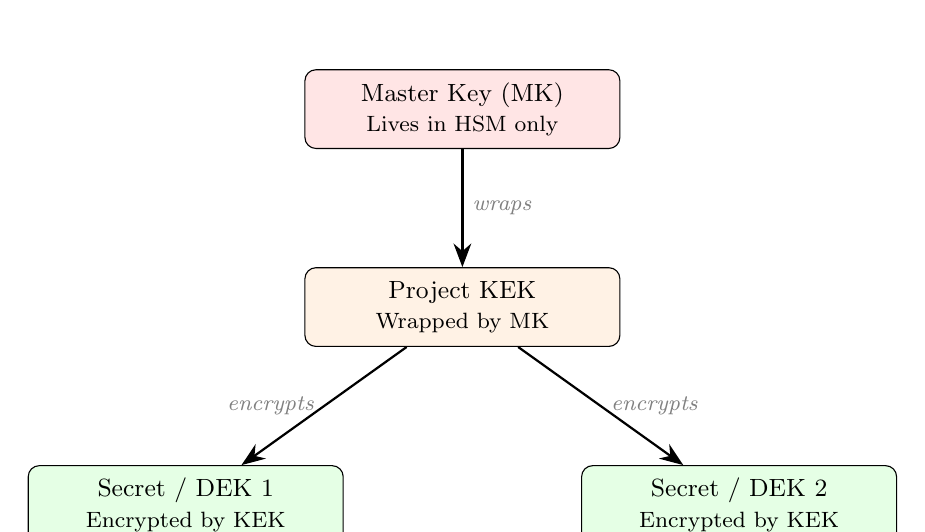
\begin{tikzpicture}[
    box/.style={rectangle, draw, rounded corners, minimum width=4cm, minimum height=1cm, align=center, font=\small},
    arrow/.style={-{Stealth[length=3mm]}, thick},
    label/.style={font=\footnotesize\itshape, text=gray}
]
    \node[box, fill=red!10] (mk) {Master Key (MK) \\ \footnotesize Lives in HSM only};
    \node[box, fill=orange!10, below=1.5cm of mk] (kek) {Project KEK \\ \footnotesize Wrapped by MK};
    \node[box, fill=green!10, below left=1.5cm and -0.5cm of kek] (dek1) {Secret / DEK 1 \\ \footnotesize Encrypted by KEK};
    \node[box, fill=green!10, below right=1.5cm and -0.5cm of kek] (dek2) {Secret / DEK 2 \\ \footnotesize Encrypted by KEK};

    \draw[arrow] (mk) -- node[right, label] {wraps} (kek);
    \draw[arrow] (kek) -- node[left, label] {encrypts} (dek1);
    \draw[arrow] (kek) -- node[right, label] {encrypts} (dek2);
\end{tikzpicture}
\caption{Envelope Encryption Hierarchy in Barbican with HSM}
\end{figure}

% ─────────────────────────────────────────────────────────────────────────
\section{Architecture and Design}

\subsection{System Components}

The complete system involves the following interacting components:

\begin{enumerate}
    \item \textbf{OpenStack Keystone:} Identity service providing authentication tokens and project (tenant) scoping.
    \item \textbf{Barbican API Server:} Receives RESTful requests to create, retrieve, list, and delete secrets. Authenticates requests via Keystone middleware.
    \item \textbf{Barbican Worker:} Asynchronous task processor handling secret encryption/decryption operations.
    \item \textbf{Secret Store Plugin (PKCS\#11):} The bridge between Barbican and the HSM. Communicates with the HSM via the PKCS\#11 interface.
    \item \textbf{HSM (Hardware Security Module):} Performs all cryptographic operations. Stores the Master Key.
    \item \textbf{Database (PostgreSQL/MySQL):} Stores encrypted secrets, wrapped KEKs, and metadata.
    \item \textbf{Message Queue (RabbitMQ):} Facilitates communication between the API server and workers.
\end{enumerate}

\subsection{Per-Tenant Key Isolation}

A critical design requirement is \textbf{per-tenant cryptographic isolation}. This is achieved as follows:

\begin{enumerate}
    \item When a tenant (identified by their OpenStack \texttt{project\_id}) stores their first secret, Barbican's PKCS\#11 plugin triggers the HSM to \textbf{generate a new KEK} specifically for that project.
    \item The HSM generates the KEK internally, wraps it using the Master Key, and returns the \textbf{wrapped KEK} to Barbican.
    \item Barbican stores the wrapped KEK in the database, associated with the \texttt{project\_id} in the \texttt{kek\_datum} table.
    \item For all subsequent secrets from that tenant, Barbican retrieves the wrapped KEK, sends it to the HSM for unwrapping, uses the unwrapped KEK to encrypt the secret (all within the HSM), and stores the encrypted secret.
    \item \textbf{Result:} Each tenant's secrets are encrypted under a unique key. Compromising one tenant's KEK does not affect other tenants. The Master Key, which protects all KEKs, never leaves the HSM.
\end{enumerate}

% ─────────────────────────────────────────────────────────────────────────
\section{Implementation Details}

\subsection{HSM Configuration}

The HSM is initialised with the following parameters:

\begin{lstlisting}[language=bash, caption={HSM Initialisation (Thales Luna Example)}]
# Initialise the HSM partition for Barbican
lunacm> partition create -name barbican_partition \
        -password <partition_password>

# Generate the Master Key (MKEK) on the HSM
lunacm> cmu generatekeypair -keytype AES \
        -keylength 256 \
        -label "barbican_hmac_key" \
        -extractable false

# Generate the HMAC key for integrity verification
lunacm> cmu generatekeypair -keytype SHA256_HMAC \
        -label "barbican_hmac_key" \
        -extractable false
\end{lstlisting}

\subsection{Barbican Configuration}

The Barbican service is configured to use the PKCS\#11 secret store plugin:

\begin{lstlisting}[language=bash, caption={barbican.conf — PKCS\#11 Plugin Configuration}]
[secretstore]
enabled_secretstore_plugins = store_crypto

[crypto]
enabled_crypto_plugins = p11_crypto

[p11_crypto_plugin]
# Path to the HSM's PKCS#11 library
library_path = /usr/lib/libCryptoki2_64.so

# HSM login credentials
login = <partition_password>

# Label of the Master KEK on the HSM
mkek_label = barbican_master_kek
mkek_length = 32

# Label of the HMAC key on the HSM
hmac_label = barbican_hmac_key

# HSM slot ID
slot_id = 1

# Token serial number (optional, for multi-slot setups)
# token_serial_number = <serial>
\end{lstlisting}

\subsection{Secret Creation Flow}

The following sequence describes the end-to-end flow when a tenant creates a secret:

\begin{enumerate}
    \item \textbf{API Request:}
\begin{lstlisting}[language=bash]
curl -X POST https://barbican.example.com/v1/secrets \
  -H "X-Auth-Token: $TOKEN" \
  -H "Content-Type: application/json" \
  -d '{
    "name": "db-encryption-key",
    "algorithm": "AES",
    "bit_length": 256,
    "mode": "CBC",
    "secret_type": "symmetric",
    "payload": "BASE64_ENCODED_KEY_MATERIAL",
    "payload_content_type": "application/octet-stream",
    "payload_content_encoding": "base64"
  }'
\end{lstlisting}

    \item \textbf{Authentication:} The Keystone middleware validates the token and extracts the \texttt{project\_id}.

    \item \textbf{KEK Lookup/Generation:}
    \begin{itemize}
        \item Barbican queries the \texttt{kek\_datum} table for an existing KEK associated with this \texttt{project\_id}.
        \item If no KEK exists (first secret for this tenant):
        \begin{enumerate}[label=(\alph*)]
            \item Barbican's PKCS\#11 plugin calls \texttt{C\_GenerateKey()} on the HSM to create a new 256-bit AES KEK.
            \item The HSM wraps the new KEK with the Master Key via \texttt{C\_WrapKey()}.
            \item The wrapped KEK is stored in the \texttt{kek\_datum} table.
        \end{enumerate}
        \item If a KEK already exists, the wrapped KEK is retrieved from the database.
    \end{itemize}

    \item \textbf{Secret Encryption:}
    \begin{enumerate}[label=(\alph*)]
        \item The wrapped KEK is sent to the HSM.
        \item The HSM unwraps it using the Master Key (\texttt{C\_UnwrapKey()}).
        \item The HSM encrypts the secret payload using the unwrapped KEK (\texttt{C\_Encrypt()}).
        \item The encrypted secret and an HMAC tag (for integrity) are returned to Barbican.
    \end{enumerate}

    \item \textbf{Persistence:} The encrypted secret, HMAC, algorithm metadata, and a reference to the KEK datum are stored in the Barbican database.

    \item \textbf{Response:} A \texttt{201 Created} response with the secret's UUID reference is returned to the tenant.
\end{enumerate}

\subsection{Secret Retrieval Flow}

\begin{enumerate}
    \item Tenant sends a GET request to \texttt{/v1/secrets/\{uuid\}/payload}.
    \item Barbican retrieves the encrypted secret and associated KEK datum from the database.
    \item The wrapped KEK and encrypted payload are sent to the HSM.
    \item The HSM unwraps the KEK, decrypts the payload, and returns the plaintext secret.
    \item The plaintext secret is returned to the tenant over TLS.
\end{enumerate}

% ─────────────────────────────────────────────────────────────────────────
\section{Security Properties}

\begin{table}[h]
\centering
\begin{tabular}{@{} l p{9cm} @{}}
\toprule
\textbf{Property} & \textbf{How It Is Achieved} \\
\midrule
Key Material Protection & Master Key never leaves the HSM; all cryptographic operations occur within HSM boundary \\
Per-Tenant Isolation & Each project has a unique KEK; secrets from different tenants cannot be decrypted with the wrong KEK \\
Defence in Depth & Even if the database is compromised, secrets are encrypted and KEKs are wrapped—unusable without HSM access \\
Integrity Verification & HMAC tags ensure that encrypted secrets have not been tampered with \\
Audit Trail & All PKCS\#11 operations are logged by both the HSM and Barbican, providing a complete audit trail \\
Regulatory Compliance & FIPS 140-2 Level 3 HSM certification satisfies PCI-DSS, HIPAA, and SOC\,2 requirements \\
\bottomrule
\end{tabular}
\caption{Security Properties Achieved via Barbican and HSM Integration}
\label{tab:barbican-security-properties}
\end{table}

% ─────────────────────────────────────────────────────────────────────────
\section{Challenges and Learnings}

\begin{enumerate}
    \item \textbf{PKCS\#11 Library Compatibility:} Different HSM vendors implement the PKCS\#11 standard with subtle variations. Debugging session management and error codes required close collaboration with vendor documentation.
    \item \textbf{HSM Session Pooling:} PKCS\#11 sessions are a limited resource. Barbican's worker pool had to be tuned to match the HSM's maximum concurrent session count, avoiding session exhaustion under load.
    \item \textbf{High Availability:} The HSM was configured in an HA pair with automatic failover. Barbican's configuration was updated to support multiple HSM addresses for seamless failover.
    \item \textbf{Performance Considerations:} HSM operations are inherently slower than software-based encryption (due to the hardware interface). Caching unwrapped KEKs in volatile HSM memory for short periods (using PKCS\#11 session objects) improved throughput without compromising security.
\end{enumerate}

% ─────────────────────────────────────────────────────────────────────────
\section{Summary}

The integration of Barbican with an HSM establishes a production-grade, multi-tenant key management system where cryptographic secrets are generated, encrypted, and stored with the highest levels of assurance. Per-tenant KEK isolation ensures that a compromise in one tenant's security posture does not cascade to others. The envelope encryption model, combined with HSM-backed key protection, satisfies stringent regulatory requirements while remaining operationally transparent to end users through Barbican's RESTful API.


% ═══════════════════════════════════════════════════════════════════════════
%     CHAPTER 3 — DISTRIBUTED PAYOUT SCHEDULING SYSTEM
% ═══════════════════════════════════════════════════════════════════════════

% ----------------------------- CHAPTER: PAYOUT ------------------------------
\chapter[Distributed Payout Scheduling]{Distributed Event-Driven Payout Scheduling System (Namma Yatri)}
\label{chap:payout}


% ─────────────────────────────────────────────────────────────────────────
\section{Introduction and Business Context}

In ride-hailing platforms, timely and accurate driver payouts are essential for driver satisfaction, retention, and platform trust. Traditionally, driver payouts are processed in \textbf{weekly batch cycles}, meaning a driver who completes a ride on Monday may not receive payment until the following Monday—a delay that is particularly burdensome in markets where drivers depend on daily cash flow.

This project addresses this challenge by designing and implementing a \textbf{distributed, event-driven payout scheduling system} for special economic zones. The system processes payouts for over \textbf{10,000 rides daily}, reducing payout latency from weekly cycles to \textbf{T+2 hours}—meaning a driver receives their payout within 2 hours of completing a ride.

% ─────────────────────────────────────────────────────────────────────────
\section{System Requirements}

The system was designed to satisfy the following requirements:

\begin{enumerate}
    \item \textbf{Low Latency:} Payout processing must complete within 2 hours of ride completion (T+2 hours).
    \item \textbf{Exactly-Once Execution:} Each ride payout must be processed exactly once—no duplicates, no missed payments.
    \item \textbf{Scalability:} The system must handle 10,000+ rides per day without degradation.
    \item \textbf{Non-Interference:} Payout scheduling must not impact ride-booking latency. The critical path (ride booking) must remain unaffected.
    \item \textbf{Fault Tolerance:} The system must gracefully handle failures (network partitions, service crashes, payment gateway timeouts) without data loss or inconsistent states.
    \item \textbf{Idempotency:} All operations must be idempotent, allowing safe retries after transient failures.
    \item \textbf{Reconciliation:} The system must support automated reconciliation for payment discrepancies.
\end{enumerate}

% ─────────────────────────────────────────────────────────────────────────
\section{Architecture Design}

\subsection{High-Level Architecture}

The system follows an \textbf{event-driven architecture} with the following components:

\begin{figure}[h]
\centering
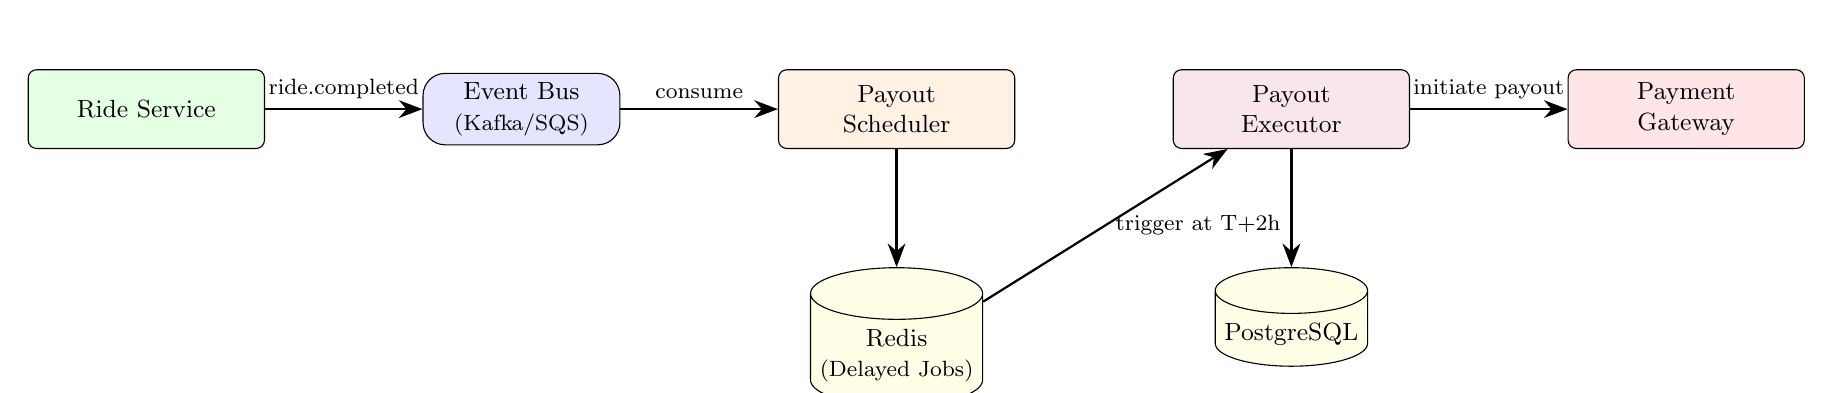
\begin{tikzpicture}[
    component/.style={rectangle, draw, rounded corners=3pt, minimum width=3cm, minimum height=1cm, align=center, font=\small},
    queue/.style={rectangle, draw, rounded corners=8pt, minimum width=2.5cm, minimum height=0.8cm, align=center, font=\small, fill=blue!10},
    db/.style={cylinder, draw, shape border rotate=90, minimum width=1.5cm, minimum height=1cm, align=center, font=\small, fill=yellow!10, aspect=0.3},
    arrow/.style={-{Stealth[length=3mm]}, thick},
    node distance=1.5cm
]
    % Components
    \node[component, fill=green!10] (ride) {Ride Service};
    \node[queue, right=2cm of ride] (event) {Event Bus \\ \footnotesize (Kafka/SQS)};
    \node[component, fill=orange!10, right=2cm of event] (scheduler) {Payout \\ Scheduler};
    \node[db, below=1.5cm of scheduler] (redis) {Redis \\ \footnotesize (Delayed Jobs)};
    \node[component, fill=purple!10, right=2cm of scheduler] (executor) {Payout \\ Executor};
    \node[component, fill=red!10, right=2cm of executor] (gateway) {Payment \\ Gateway};
    \node[db, below=1.5cm of executor] (db) {PostgreSQL};

    % Arrows
    \draw[arrow] (ride) -- node[above, font=\footnotesize] {ride.completed} (event);
    \draw[arrow] (event) -- node[above, font=\footnotesize] {consume} (scheduler);
    \draw[arrow] (scheduler) -- (redis);
    \draw[arrow] (redis) -- node[right, font=\footnotesize] {trigger at T+2h} (executor);
    \draw[arrow] (executor) -- node[above, font=\footnotesize] {initiate payout} (gateway);
    \draw[arrow] (executor) -- (db);
\end{tikzpicture}
\caption{High-Level Architecture of the Payout Scheduling System}
\end{figure}

\subsection{Component Responsibilities}

\begin{description}
    \item[Ride Service:] Emits a \texttt{ride.completed} event to the event bus upon ride completion. This is a fire-and-forget operation that adds zero latency to the ride-booking critical path.

    \item[Event Bus (Kafka/SQS):] Provides durable, ordered message delivery. Serves as a decoupling layer between the ride service and the payout subsystem.

    \item[Payout Scheduler:] Consumes \texttt{ride.completed} events and schedules a delayed payout job in Redis with a 2-hour delay. Applies per-ride locking to prevent duplicate scheduling.

    \item[Redis (Delayed Job Store):] Stores scheduled payout jobs using sorted sets (\texttt{ZADD}) with the execution timestamp as the score. Provides O(1) scheduling and O(log\,N) retrieval of due jobs.

    \item[Payout Executor:] A worker process that polls Redis for jobs whose execution timestamp has passed. Processes payouts with exactly-once semantics using idempotent state transitions.

    \item[Payment Gateway (Paytm EDC):] The external payment provider. Handles the actual fund transfer to the driver's account.

    \item[PostgreSQL:] Persistent storage for payout records, state transitions, and audit logs.
\end{description}

% ─────────────────────────────────────────────────────────────────────────
\section{Detailed Design}

\subsection{Redis-Backed Delayed Job Scheduler}

The delayed job scheduler is the core innovation enabling the T+2-hour payout guarantee. It leverages Redis sorted sets for efficient scheduling:

\begin{lstlisting}[language=Python, caption={Delayed Job Scheduling Logic}]
import redis
import time
import json
import hashlib

r = redis.Redis(host='redis-cluster', port=6379, db=0)

PAYOUT_QUEUE = "payout:delayed_jobs"
PAYOUT_LOCK_PREFIX = "payout:lock:"
PAYOUT_DELAY_SECONDS = 7200  # 2 hours

def schedule_payout(ride_id, driver_id, amount, zone_id):
    """
    Schedule a payout job with T+2 hour delay.
    Uses per-ride locking for exactly-once scheduling.
    """
    lock_key = f"{PAYOUT_LOCK_PREFIX}{ride_id}"

    # Acquire per-ride lock (NX = set if not exists, EX = TTL)
    if not r.set(lock_key, "locked", nx=True, ex=86400):
        # Lock already exists => payout already scheduled
        return False  # Idempotent: no duplicate scheduling

    execution_time = time.time() + PAYOUT_DELAY_SECONDS
    job = json.dumps({
        "ride_id": ride_id,
        "driver_id": driver_id,
        "amount": amount,
        "zone_id": zone_id,
        "scheduled_at": time.time(),
        "idempotency_key": hashlib.sha256(
            f"{ride_id}:{driver_id}".encode()
        ).hexdigest()
    })

    # ZADD with score = execution timestamp
    r.zadd(PAYOUT_QUEUE, {job: execution_time})
    return True
\end{lstlisting}

\textbf{Key design decisions:}
\begin{itemize}
    \item \textbf{Per-Ride Locking (\texttt{SET NX}):} Ensures that even if the \texttt{ride.completed} event is delivered multiple times (at-least-once delivery), the payout is scheduled only once. The lock has a 24-hour TTL for automatic cleanup.
    \item \textbf{O(1) Scheduling:} \texttt{ZADD} is an O(log\,N) operation on the sorted set, but since jobs are append-mostly, the amortised cost is effectively O(1).
    \item \textbf{Idempotency Key:} A deterministic hash of \texttt{ride\_id} and \texttt{driver\_id} serves as a deduplication key at the payment gateway level.
\end{itemize}

\subsection{Payout Executor with Idempotent State Management}

The executor processes due jobs with a carefully designed state machine:

\begin{center}
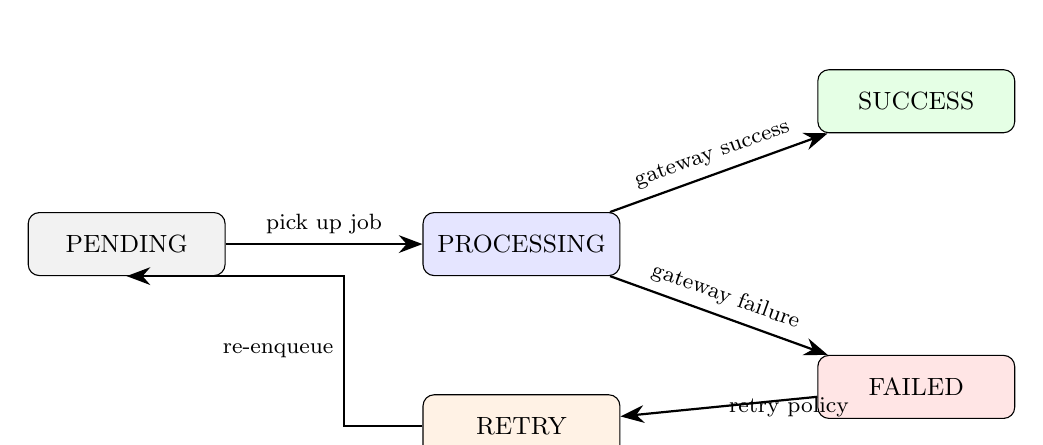
\begin{tikzpicture}[
    state/.style={rectangle, draw, rounded corners, minimum width=2.5cm, minimum height=0.8cm, align=center, font=\small},
    arrow/.style={-{Stealth[length=3mm]}, thick},
    node distance=2cm
]
    \node[state, fill=gray!10] (pending) {PENDING};
    \node[state, fill=blue!10, right=2.5cm of pending] (processing) {PROCESSING};
    \node[state, fill=green!10, above right=1cm and 2.5cm of processing] (success) {SUCCESS};
    \node[state, fill=red!10, below right=1cm and 2.5cm of processing] (failed) {FAILED};
    \node[state, fill=orange!10, below=1.5cm of processing] (retry) {RETRY};

    \draw[arrow] (pending) -- node[above, font=\footnotesize] {pick up job} (processing);
    \draw[arrow] (processing) -- node[above, font=\footnotesize, sloped] {gateway success} (success);
    \draw[arrow] (processing) -- node[above, font=\footnotesize, sloped] {gateway failure} (failed);
    \draw[arrow] (failed) -- node[right, font=\footnotesize] {retry policy} (retry);
    \draw[arrow] (retry.west) -- +(-1,0) |- node[left, font=\footnotesize, pos=0.25] {re-enqueue} (pending.south);
\end{tikzpicture}
\end{center}

\begin{lstlisting}[language=Python, caption={Payout Executor with State Machine}]
def execute_due_payouts():
    """
    Poll for jobs whose execution time has passed.
    Process with exactly-once semantics.
    """
    now = time.time()

    # ZRANGEBYSCORE: get all jobs with score <= now
    due_jobs = r.zrangebyscore(
        PAYOUT_QUEUE, '-inf', now, start=0, num=100
    )

    for job_data in due_jobs:
        job = json.loads(job_data)
        ride_id = job['ride_id']

        # Begin state transition: PENDING -> PROCESSING
        if not transition_state(ride_id, 'PENDING', 'PROCESSING'):
            continue  # Already processing or completed

        try:
            # Call payment gateway with idempotency key
            result = initiate_payout(
                driver_id=job['driver_id'],
                amount=job['amount'],
                idempotency_key=job['idempotency_key']
            )

            if result.success:
                transition_state(ride_id, 'PROCESSING', 'SUCCESS')
                r.zrem(PAYOUT_QUEUE, job_data)  # Remove from queue
            else:
                handle_failure(job, result)

        except Exception as e:
            transition_state(ride_id, 'PROCESSING', 'FAILED')
            schedule_retry(job, retry_count=job.get('retries', 0))

def transition_state(ride_id, from_state, to_state):
    """
    Atomic state transition using database CAS
    (Compare-And-Swap) semantics.
    """
    result = db.execute("""
        UPDATE payout_jobs
        SET state = %s, updated_at = NOW()
        WHERE ride_id = %s AND state = %s
    """, (to_state, ride_id, from_state))
    return result.rowcount == 1  # True if transition succeeded
\end{lstlisting}

\subsection{Paytm EDC Integration}

The system integrates with \textbf{Paytm EDC (Electronic Data Capture)} terminals—Android-based Point-of-Sale (POS) devices—for processing in-zone payments. The integration involves:

\subsubsection{Type-Safe API Design}

All API interactions with the Paytm EDC gateway are modelled using strongly-typed request/response structures:

\begin{lstlisting}[language=Python, caption={Type-Safe Payment API Models}]
from dataclasses import dataclass
from enum import Enum
from typing import Optional
from decimal import Decimal

class PaymentStatus(Enum):
    INITIATED = "INITIATED"
    SUCCESS = "SUCCESS"
    FAILED = "FAILED"
    REFUNDED = "REFUNDED"
    PENDING = "PENDING"

@dataclass(frozen=True)
class PayoutRequest:
    ride_id: str
    driver_id: str
    amount: Decimal
    currency: str = "INR"
    idempotency_key: str = ""
    zone_id: str = ""

@dataclass(frozen=True)
class PayoutResponse:
    transaction_id: str
    status: PaymentStatus
    amount: Decimal
    timestamp: str
    error_code: Optional[str] = None
    error_message: Optional[str] = None
\end{lstlisting}

\subsubsection{Reconciliation Engine}

Automated reconciliation ensures consistency between the platform's records and the payment gateway's records:

\begin{lstlisting}[language=Python, caption={Reconciliation Logic}]
def reconcile_payouts(date):
    """
    Daily reconciliation between internal records
    and gateway settlement reports.
    """
    internal_records = db.query("""
        SELECT ride_id, amount, status, transaction_id
        FROM payout_jobs
        WHERE DATE(created_at) = %s AND status = 'SUCCESS'
    """, (date,))

    gateway_records = paytm_api.get_settlement_report(date)

    # Build lookup maps
    internal_map = {r.transaction_id: r for r in internal_records}
    gateway_map = {r.txn_id: r for r in gateway_records}

    discrepancies = []

    # Check for records in our DB but not in gateway
    for txn_id, record in internal_map.items():
        if txn_id not in gateway_map:
            discrepancies.append({
                'type': 'MISSING_AT_GATEWAY',
                'ride_id': record.ride_id,
                'amount': record.amount
            })

    # Check for amount mismatches
    for txn_id in internal_map.keys() & gateway_map.keys():
        if internal_map[txn_id].amount != gateway_map[txn_id].amount:
            discrepancies.append({
                'type': 'AMOUNT_MISMATCH',
                'ride_id': internal_map[txn_id].ride_id,
                'internal_amount': internal_map[txn_id].amount,
                'gateway_amount': gateway_map[txn_id].amount
            })

    return discrepancies
\end{lstlisting}

\subsubsection{Refund Handling}

For failed transactions where the payment was debited but the payout was not completed, the system implements automated refund processing:

\begin{lstlisting}[language=Python, caption={Refund Handling for Failed Transactions}]
def handle_failed_transaction(job, gateway_response):
    """
    If the gateway reports a debit but the payout failed,
    initiate a refund.
    """
    if (gateway_response.status == PaymentStatus.FAILED and
            gateway_response.error_code == "DEBIT_SUCCESS_CREDIT_FAIL"):

        refund_result = paytm_api.initiate_refund(
            original_txn_id=gateway_response.transaction_id,
            amount=job['amount'],
            reason="CREDIT_FAILURE_AUTO_REFUND"
        )

        db.execute("""
            INSERT INTO refund_log
            (ride_id, original_txn_id, refund_txn_id,
             amount, status, created_at)
            VALUES (%s, %s, %s, %s, %s, NOW())
        """, (job['ride_id'],
              gateway_response.transaction_id,
              refund_result.refund_id,
              job['amount'],
              refund_result.status))
\end{lstlisting}

\subsubsection{Status Polling}

To handle asynchronous payment processing, the system implements robust status polling with exponential backoff:

\begin{lstlisting}[language=Python, caption={Payment Status Polling with Backoff}]
import time

def poll_payment_status(transaction_id, max_attempts=10):
    """
    Poll the payment gateway for final transaction status.
    Uses exponential backoff to avoid overwhelming the gateway.
    """
    base_delay = 1  # seconds
    for attempt in range(max_attempts):
        response = paytm_api.check_status(transaction_id)

        if response.status in (PaymentStatus.SUCCESS,
                               PaymentStatus.FAILED):
            return response  # Terminal state reached

        # Exponential backoff: 1s, 2s, 4s, 8s, ...
        delay = base_delay * (2 ** attempt)
        delay = min(delay, 60)  # Cap at 60 seconds
        time.sleep(delay)

    # Max attempts exhausted; mark for manual review
    return PayoutResponse(
        transaction_id=transaction_id,
        status=PaymentStatus.PENDING,
        amount=Decimal('0'),
        timestamp=str(time.time()),
        error_message="Status polling timed out"
    )
\end{lstlisting}

% ─────────────────────────────────────────────────────────────────────────
\section{Performance Characteristics}

\begin{table}[h]
\centering
\begin{tabular}{@{} l l @{}}
\toprule
\textbf{Metric} & \textbf{Value} \\
\midrule
Daily Ride Volume & 10,000+ rides \\
Payout Latency & T+2 hours (previously weekly) \\
Scheduling Throughput & O(1) per ride (Redis ZADD) \\
Exactly-Once Guarantee & Per-ride locks + idempotent state machine \\
Impact on Ride Booking Latency & Zero (async event-driven) \\
Retry Policy & Exponential backoff, max 5 retries \\
Reconciliation Frequency & Daily automated + weekly manual audit \\
\bottomrule
\end{tabular}
\caption{Performance Characteristics of the Distributed Payout System}
\label{tab:payout-performance}
\end{table}

% ─────────────────────────────────────────────────────────────────────────
\section{Challenges and Learnings}

\begin{enumerate}
    \item \textbf{Redis Persistence vs.\ Performance:} Redis' in-memory nature provides speed but risks data loss. The system uses Redis with AOF (Append-Only File) persistence and periodic RDB snapshots. Additionally, all job metadata is persisted to PostgreSQL before being enqueued in Redis, providing a recovery path.

    \item \textbf{Clock Skew in Distributed Systems:} The delayed job mechanism relies on timestamps. In a multi-node deployment, clock skew between nodes could cause premature or delayed job execution. This was mitigated by using NTP synchronisation and accepting a $\pm$500ms tolerance window.

    \item \textbf{Payment Gateway Idempotency:} Not all payment gateways natively support idempotency keys. For Paytm EDC, the idempotency contract was verified empirically, and the system was designed to handle non-idempotent edge cases via reconciliation.

    \item \textbf{Handling Zone-Specific Regulations:} Special economic zones have different tax and regulatory requirements. The system parameterises payout calculations based on zone configuration, allowing per-zone customisation without code changes.

    \item \textbf{Monitoring and Alerting:} Custom metrics were added:
    \begin{itemize}
        \item \texttt{payout.scheduled.count} — Number of payouts scheduled per minute
        \item \texttt{payout.executed.count} — Number of payouts executed per minute
        \item \texttt{payout.failed.count} — Number of failed payouts (triggers alert if > threshold)
        \item \texttt{payout.latency.p99} — 99th percentile payout processing time
    \end{itemize}
\end{enumerate}

% ─────────────────────────────────────────────────────────────────────────
\section{Summary}

The distributed payout scheduling system transforms driver payments from a slow, batch-oriented process into a near-real-time, event-driven pipeline. Key achievements include:

\begin{itemize}
    \item \textbf{97\%+ reduction in payout latency} (weekly $\to$ 2 hours)
    \item \textbf{Exactly-once payment processing} via per-ride locking and idempotent state machines
    \item \textbf{Zero impact on ride-booking critical path} through asynchronous event-driven architecture
    \item \textbf{Automated reconciliation and refund handling} eliminating manual intervention for payment discrepancies
    \item \textbf{Production-proven at scale} serving 10,000+ rides daily
\end{itemize}


% ═══════════════════════════════════════════════════════════════════════════
%                          CONCLUSION

% ----------------------------- CHAPTER: POSTGRES ON K8S/OPENSTACK -----------
\chapter[PostgreSQL on Kubernetes/OpenStack]{Self-Directed Project: PostgreSQL on Kubernetes/OpenStack}
\label{chap:postgres-k8s}

\section{Motivation and Scope}

Industry teams routinely operate Postgres on Kubernetes on top of OpenStack-managed VMs in production, but the full stack --- from bare metal up through the database --- is rarely available to a single engineer to exercise end-to-end. This self-directed project replicated that stack on a single workstation (an Intel i9-14900) with sufficient fidelity that it could be used as both a learning vehicle and a reproducible testbed for failure-injection experiments.

The project produced three engineering deliverables:

\begin{enumerate}[leftmargin=*]
    \item A five-layer nested virtualisation stack tuned for write-heavy database workloads.
    \item A zero-touch, end-to-end automation pipeline that brings a fresh OpenStack tenant from empty to a running, highly-available PostgreSQL cluster in roughly 12 minutes.
    \item A Zero-Trust secret delivery framework with a Go-based broker and a Python SDK that VMs use to fetch their secrets at first boot without long-lived credentials.
\end{enumerate}

\section{Five-Layer Nested Virtualisation Stack}

The stack consists of, from the bottom up:

\begin{description}[leftmargin=*]
    \item[Layer 1 --- Bare metal:] Intel i9-14900, 24 cores (8 P-cores + 16 E-cores), 128\,GB DDR5, NVMe storage.
    \item[Layer 2 --- KVM host:] Linux + libvirt with VT-x and EPT enabled; nested virtualisation toggled on (\texttt{kvm-intel.nested=1}).
    \item[Layer 3 --- OpenStack control plane:] A single-host OpenStack deployment (Nova, Neutron, Cinder, Glance, Keystone, Barbican) running inside a single privileged VM. Storage backed by Cinder over Ceph; networking via OVN.
    \item[Layer 4 --- Kubernetes:] HA Kubernetes cluster (3 control-plane + 3 worker nodes) provisioned as OpenStack instances, control plane behind a kube-vip virtual IP.
    \item[Layer 5 --- PostgreSQL:] CloudNativePG-managed Postgres cluster (1 primary + 2 synchronous replicas) running on the K8s layer, with PVCs backed by Cinder (and, transitively, by the Layer 1 NVMe).
\end{description}

\subsection{Performance Tuning}

Naive nested virtualisation is slow: every database write traverses five virtual block devices and four network stacks. Two tuning passes recovered the bulk of the loss:

\begin{itemize}[leftmargin=*]
    \item \textbf{NUMA-aware CPU pinning.} The 8 P-cores were partitioned across the OpenStack control VM, the K8s control-plane VMs, and the K8s workers. Each level was given an exclusive, NUMA-pinned set of vCPUs via libvirt's \texttt{<cputune>} and OpenStack's \texttt{hw:cpu\_policy=dedicated}. Cross-NUMA traffic was eliminated for the database workers.
    \item \textbf{16\,GB hugepages.} Both the OpenStack VMs and the database PVCs were backed by 1\,GB hugepages, totalling 16\,GB pinned. This reduced TLB pressure visibly and stabilised \texttt{pgbench} TPS variance.
\end{itemize}

The combined effect on a TPC-B-like \texttt{pgbench} workload was an approximately \textbf{50\,\%} increase in write TPS over the un-tuned baseline.

\section{Zero-Touch Cluster Provisioning}

The objective was that running a single command (\texttt{make cluster}) should yield a verified-healthy HA Postgres cluster, with no operator interaction beyond entering an SSH key.

The pipeline composes three open-source projects:

\begin{description}[leftmargin=*]
    \item[Cluster API for OpenStack (CAPO):] declarative provisioning of K8s clusters as OpenStack workloads. CAPO consumes a \texttt{Cluster}, \texttt{OpenStackCluster}, and \texttt{KubeadmControlPlane} manifest and reconciles the live state of the OpenStack tenant against them.
    \item[CloudNativePG (CNPG):] a Kubernetes operator that provisions and manages PostgreSQL clusters as first-class K8s resources. The operator handles streaming replication, synchronous-replica election, automatic failover, and PITR via base backups + WAL archive.
    \item[A small Make/shell wrapper:] orchestrates the OpenStack tenant bootstrap, applies the CAPI manifests, waits for cluster readiness, then applies the CNPG manifests.
\end{description}

\subsection{Time Breakdown}

End-to-end provisioning of an empty OpenStack tenant to a healthy 3-replica Postgres cluster takes roughly \textbf{12 minutes} on the i9-14900:

\begin{itemize}[leftmargin=*]
    \item OpenStack tenant bootstrap (network, security groups, image): $\sim$1 min
    \item Control-plane VM creation + cloud-init: $\sim$3 min
    \item Worker VM creation + cloud-init: $\sim$3 min
    \item kubeadm + CNI bring-up: $\sim$2 min
    \item CNPG operator install + Postgres cluster creation: $\sim$3 min
\end{itemize}

\subsection{Failover Behaviour}

A controlled \texttt{kill -9} of the Postgres primary results in CNPG promoting a synchronous replica within \textbf{$\sim$7\,seconds}, with \textbf{RPO = 0} confirmed by replaying the test workload against the new primary and observing no missing transactions. The same drill against an entire K8s control-plane node (simulated power loss of one of the three) similarly recovered within the kube-vip + etcd liveness budget without data loss.

\section{Zero-Trust Secret Delivery Framework}

The provisioning pipeline must hand secrets (database passwords, certificate keys, OAuth client credentials) to fresh VMs without requiring those VMs to ship pre-baked credentials. The constraint is the well-known \emph{secret-zero} bootstrapping problem.

\subsection{Architecture}

A small Go-based broker, \texttt{osvault-broker}, sits adjacent to the OpenBao cluster (Chapter~\ref{chap:openbao}). The flow is:

\begin{enumerate}[leftmargin=*]
    \item A fresh VM, on first boot, calls the OpenStack \textbf{Instance Metadata Service (IMDS)} for a signed identity document containing \texttt{instance\_id}, \texttt{project\_id}, and a Nova-signed assertion of liveness.
    \item The VM sends this assertion to \texttt{osvault-broker} over the local OpenStack tenant network.
    \item The broker validates the IMDS signature, looks up the instance's role in OpenBao's policy DB, and mints a short-lived (5\,min) \textbf{RS256-signed JWT} carrying the appropriate OpenBao token.
    \item The VM presents the JWT to OpenBao and receives its scoped secrets.
\end{enumerate}

No long-lived secret material is ever placed in cloud-init userdata or in the VM image. The trust chain rests on the IMDS signing key (rotated weekly) and the broker's RSA key (held only in OpenBao's transit engine).

\subsection{Custom Python SDK: \texttt{osvault}}

To make consumption ergonomic, a small Python SDK named \texttt{osvault} wraps the broker handshake. A typical first-boot script looks like:

\begin{lstlisting}[language=Python, caption={First-boot secret retrieval via osvault}]
from osvault import VaultClient

client = VaultClient.from_imds()        # auto-discovers IMDS, fetches RS256 JWT
db = client.get("postgres/credentials") # short-lived DB password
tls = client.get("tls/server-cert")     # private key + cert chain

write_pgpass(db.username, db.password)
write_tls_pair(tls.cert, tls.key)
\end{lstlisting}

The SDK handles JWT renewal, retries on transient broker unavailability, and clears all secret material from memory after use (\texttt{ctypes.memset} on the underlying buffers).

\section{Outcomes and Reusability}

The stack is reproducible from a single Git repository and a Make target. It has served as a sandbox for several follow-on experiments: chaos-style failure injection on the Postgres layer, latency profiling of nested networking, and dry-runs of OpenStack upgrades against a representative tenant. Beyond personal learning, the resulting Make pipeline and the \texttt{osvault} SDK are reusable artifacts: the pipeline has been adopted internally as the canonical way to spin up disposable test clusters, and the SDK has been packaged as an internal Python wheel.


% ----------------------------- CHAPTER: CONCLUSION --------------------------
\chapter{Conclusion}
\label{chap:conclusion}

\section{Summary}

This internship year exposed me to three distinct strata of the production distributed-systems stack: \emph{block storage} (Lightbits NVMe/TCP replacing CEPH at Juspay), \emph{in-process state management} (the two-tier caching layer for high-traffic payment APIs), and \emph{secrets infrastructure} (the Shamir-secret-sharing-based OpenBao cluster, with the supporting Barbican KMS + HSM integration). In parallel, the open-source contribution to Namma Yatri delivered a distributed event-driven payout scheduler under live production traffic, and the self-directed PostgreSQL on Kubernetes/OpenStack project closed the loop by exercising the full stack from bare metal to database on a single workstation.

The headline numbers across these projects --- 4$\times$ storage efficiency on Lightbits, 4.1\,\% cross-node call reduction and 11.2\,\% p95 latency reduction on caching, 7-second automatic failover on the K8s/Postgres stack with RPO=0, and the migration of Namma Yatri driver payouts from weekly cycles to T+2 hours --- are individually meaningful but, taken together, point to a recurring engineering principle: the largest wins came not from new abstractions but from \emph{taking correctness seriously while doing more with fewer machines}.

\section{Skills Developed}

\begin{itemize}[leftmargin=*]
    \item \textbf{Production distributed-systems engineering:} writing code that runs on real money-moving traffic; understanding tail latency, blast radius, and recovery as first-class design constraints.
    \item \textbf{Cross-stack debugging:} reasoning about a single transaction's path across application, cache, Redis, OpenStack volume, and Lightbits storage --- and being able to attribute latency to any layer.
    \item \textbf{Open-source collaboration:} the Namma Yatri PR went through public review with the community and a maintainer who set a high bar for design clarity, idempotency, and test coverage.
    \item \textbf{Cryptographic engineering hygiene:} Shamir secret sharing, RS256 JWT discipline, mlock-based memory protection, and the operational drills that go with self-custodial key material.
    \item \textbf{Systems-level performance tuning:} NUMA-aware CPU pinning, hugepages, nested virtualisation, and the empirical method of validating each tuning step against a reproducible benchmark.
\end{itemize}

\section{Future Directions}

\begin{itemize}[leftmargin=*]
    \item Extend the caching framework with a contention layer that handles single-resource state safely; this is the subject of the parallel B.Tech project report.
    \item Generalise the OpenBao broker into a small, reusable open-source project (currently internal-only) so other teams running OpenStack can adopt the pattern.
    \item Run the PostgreSQL on K8s/OpenStack pipeline as a chaos-engineering testbed: scripted failure injection at each of the five virtualisation layers, with end-to-end correctness invariants.
\end{itemize}


% ============================== BIBLIOGRAPHY =================================
\begin{thebibliography}{99}

\bibitem{lightbits}
Lightbits Labs, ``LightOS Technical Documentation,''
\url{https://www.lightbitslabs.com/resources/}

\bibitem{ceph}
Weil, S.A., et al.,
``Ceph: A Scalable, High-Performance Distributed File System,''
\textit{Proceedings of the 7th Symposium on Operating Systems Design and Implementation (OSDI)}, 2006.

\bibitem{nvmetcp}
NVM Express, Inc.,
``NVMe over Fabrics Specification,''
\url{https://nvmexpress.org/specifications/}

\bibitem{barbican}
OpenStack Barbican,
``Key Manager Service Documentation,''
\url{https://docs.openstack.org/barbican/latest/}

\bibitem{pkcs11}
RSA Laboratories,
``PKCS \#11: Cryptographic Token Interface Standard,''
\url{https://www.cryptsoft.com/pkcs11doc/}

\bibitem{fips140}
NIST,
``FIPS 140-2: Security Requirements for Cryptographic Modules,''
2001.

\bibitem{redis}
Redis Ltd.,
``Redis Sorted Sets Documentation,''
\url{https://redis.io/docs/data-types/sorted-sets/}

\bibitem{kafka}
Apache Software Foundation,
``Apache Kafka Documentation,''
\url{https://kafka.apache.org/documentation/}

\bibitem{paytm}
Paytm,
``EDC Payment Gateway API Documentation,''
\url{https://developer.paytm.com/}

\bibitem{idempotency}
Helland, P.,
``Idempotence Is Not a Medical Condition,''
\textit{Communications of the ACM}, vol.\ 55, no.\ 5, 2012.

\bibitem{shamir1979}
Shamir, A.,
``How to Share a Secret,''
\textit{Communications of the ACM}, vol.\ 22, no.\ 11, pp.\ 612--613, 1979.

\bibitem{ongaro2014raft}
Ongaro, D. and Ousterhout, J.,
``In Search of an Understandable Consensus Algorithm (Raft),''
\textit{Proceedings of the 2014 USENIX Annual Technical Conference}, 2014.

\bibitem{openbao}
OpenBao Maintainers,
``OpenBao: Open Source Secrets Management,''
\url{https://openbao.org/}, 2025.

\bibitem{capi}
Kubernetes SIGs,
``Cluster API and Cluster API Provider OpenStack (CAPO),''
\url{https://cluster-api.sigs.k8s.io/}, 2025.

\bibitem{cnpg}
EnterpriseDB,
``CloudNativePG: Postgres Operator for Kubernetes,''
\url{https://cloudnative-pg.io/}, 2025.

\bibitem{kumar2024caching}
Kumar, A., et al.,
``Comparative Analysis of Distributed Caching Algorithms,''
arXiv:2504.02220, 2024.

\bibitem{nammayatri}
Namma Yatri Project,
``Open-Source Mobility Platform,''
\url{https://github.com/nammayatri/nammayatri}, 2026.

\end{thebibliography}

\end{document}
